\newcommand{\hmsscore}{\mathrm{HMS}}
\newcommand{\contextscore}{\mathrm{ctx}_\mathrm{F1}}
\newcommand{\variablescore}{\mathrm{var}_\mathrm{F1}}
\newcommand{\relationscore}{\mathrm{rel}_\mathrm{acc}}

\section{\discoverybench}
\label{sec:discovery_bench}

We now introduce a novel benchmark, \discoverybench{}, for discovering data-driven hypotheses. In this benchmark, a \emph{data-driven discovery task} is defined as follows: Given one or more task dataset(s)
% \ashish{added notation:}
$D$ and a discovery goal $G$, derive a hypothesis $h = \psi(c,v,r)$ addressing $G$ with the highest specificity for the context $c$, variables $v$, and relationship $r$ supported by $D$. Optionally, a workflow of deriving such a hypothesis can be outputted to augment information already present in the hypothesis. \discoverybench{} has two components: \textbf{\real}
% \ashish{seems odd to call the benchmarks just Real and Synth. Alternatives? \textsc{DB-\real}? \textsc{DBench-\real}? \textsc{Disc-\real}?} 
encompassing data-driven hypotheses and workflows derived from published scientific papers and \textbf{\synth} capturing systemic variations in data-driven hypotheses and workflows obtained from synthetically generated datasets. We release our dataset under the ODC-BY license: \url{https://github.com/allenai/discoverybench}.

% \ashish{not sure where this would go (would there be a dataset stats table?), but it would help to state how many datasets are involved in total (in \real{} and in \synth{}), and generally how many tasks require 1 dataset vs.\ more.}

\subsection{\real: Collecting data-driven hypotheses in the wild}

Our goal is to replicate the scientific process undertaken by researchers to search for and validate a hypothesis from one or more datasets. We focus on six scientific domains where data-driven research is the cornerstone of scientific progress: sociology, biology, humanities, economics, engineering, and meta-science. Our data collection follows either a \textbf{data-first} or \textbf{code-first} approach.

For the \textbf{data-first approach}: 1) we filter papers based on open public datasets ($D$) such as National Longitudinal Surveys (NLS), Global Biodiversity Information Facility (GBIF), and World Bank Open Data (WBOD) that have workflow details; 2) we then try to replicate these workflows in Python. For this data-first approach, replication took up to 90 person-hours per dataset, often (30\%) not resulting in success. This highlights building data-driven discovery benchmarks from real studies is not only challenging and time-consuming, but automating discovery can also be key for scientific progress and reproducibility. 

% for the GBIF dataset, where specialized domain knowledge and tools led to higher complexity. All papers replicated in the NLS dataset were included, while less than half of the papers in specialized datasets like GBIF and WBOD were added to \discoverybench{}. 


The data-first approach by design is limited to well-known aforementioned public datasets. To improve diversity in domains, datasets ($D$), and workflows, we also adopted a \textbf{code-first approach} to look beyond popular public datasets. 
% enhance the diversity of the datasets ($D$) and therefore domains and workflows as well. \dhruv{Unsure how 'diversity' is increased by this approach.} \harshit{diversity is introduced by exploring beyond well known public datasets mentioned above, which in turn leads to domain and workflow diversity. @bodhi this is a valid point let us see how we can add it here to contrast from paper-first} \ashish{+1. would be helpful to explain; it's unclear at the moment.}
In this approach, we 1) search for code repositories based on scientific papers with available datasets and 2) attempt to replicate them in Python with existing code or from scratch with interpretation of the associated paper. We looked at 785 data points in Zenodo, EU's Open Research Repository, with a filter for computational notebooks. Over 85\% of the repositories either had missing code, code that could not be easily translated to Python, or a proprietary/non-open dataset. We finalized a candidate list of 14 repositories, but in the end, 3 of them passed all our checks for their hypotheses to be included in the benchmark\footnote{Some repositories include hypotheses from multiple papers as their background.}. 
% verify if the repository has no missing dataset or methods. If replication proves unsuccessful, we attempt to reimplement the workflows from scratch in Python based on our interpretation of the associated paper. Otherwise, we exclude them entirely.

%1) Search for papers (in paper-first) or code repositories (code-first) for a specific domain, 2) filter papers/repositories based on the dataset ($D$) and implementation code availability, 3) then, for each filtered paper/repositories, we attempt to replicate the derivation of a hypothesis in Python by either using available code or implementing it from scratch. In cases where code did not run, or replication was unsuccessful due to missing code \harshit{i think missing code is also accompanied by missing data or partial data as well as lack of domain knowledge}, we re-implement from scratch using the implementation workflow described in the paper. To ensure data availability for paper-first approach, we mainly targeted papers written on large, public datasets such as NLS, Global Biodiversity Information Facility, and World Bank Open Data.
% \harshit{there was no available code for paper first approach except in one case (pathways) where the code did not run. that is why we moved to code first approach, instead of trying to understand the paper, then replicate - first check if the code runs and then go from there},

% \bodhi{@harshit, Can you comment 1 sentence about the practical diffs in outcomes of paper and code-first approach?}
% \harshit{this is not very readable or easy to distinguish the difference between code first or paper first approach}
% \harshit{this writeup also strips away all the issues faced in understanding and replicating papers in a wide range of domains with for paper first approach. for code first approach it does not cover the key concerns of finding code with full datasets. i think it is quite important to explain this practical difficulty else a valid question on, else the expectation of numbers of hypotheses would be similar to swe-bench which just crawls github issues}
% \bodhi{I understand, but we need to explain that systematically. How about telling the hours required to replicate each paper/workflow? Can you say any numbers on successful find vs total search? That will also explain the complexity. We need brevity here, details can go in appendix}
% \harshit{yes! we give systematic numbers for paper search + replication for NLS, GBIF, World Bank. For code first we have numbers on how many repos were scanned, how many we tried, and how many finally made in. will that work?}

\begin{figure}[t!]
    \centering
    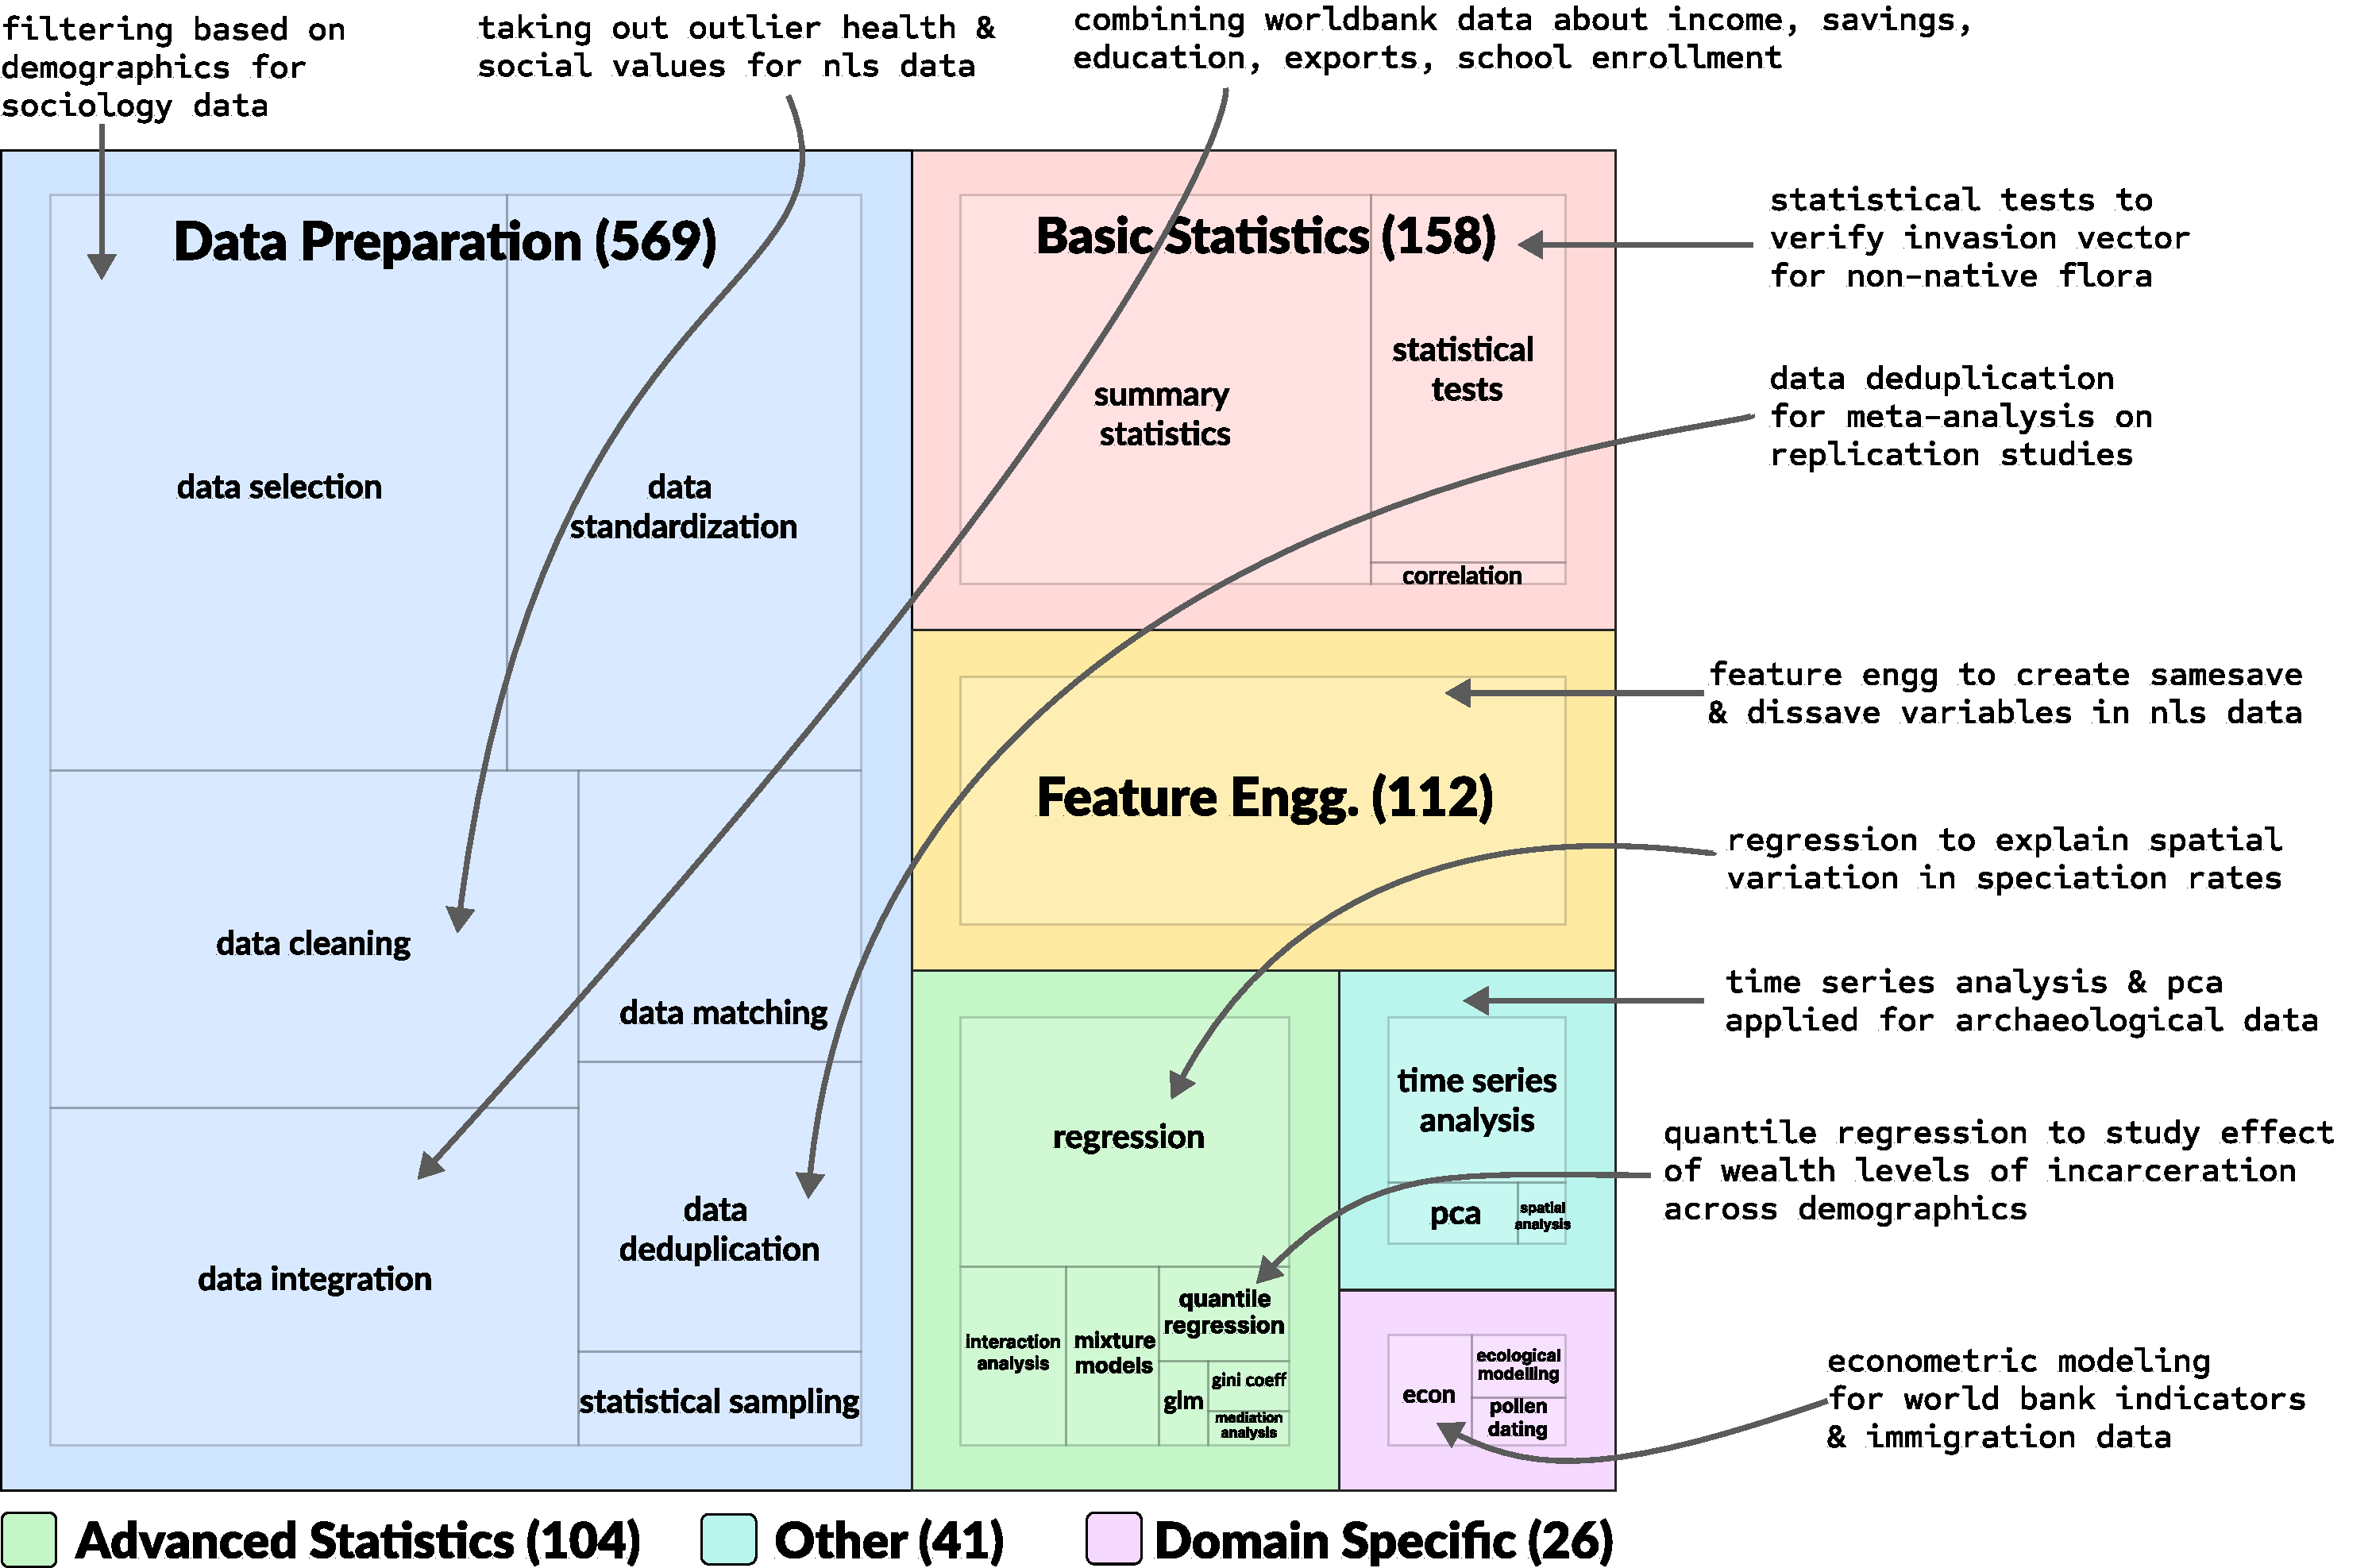
\includegraphics[trim=0 0 0 0,clip, width=0.95\textwidth]{figures/fig2-glance.pdf}
    \caption{\small Workflow categories in \real{} with representative examples.}
    \label{fig:fig2}
    \vspace{-3mm}
\end{figure}




% (note: ). \tushar{This workflow was a bit complicated to follow. Also the interleaving of code first and paper first also makes it harder. Could we describe each approach independently? Also could we show the pipeline for code first and paper first with an image (even if appendix) with associated time taken or filter \%s where appropriate?} \ashish{In case it helps, I split the above paragraph into two parts. But generally, yes, it might be better to first fully describe the paper-first approach in one paragraph, and then the code-first in the 2nd paragraph (no interleaving).}\harshit{yes, that will flow much better - made the change}

% \textbf{Code-first:} 1) Search for code repositories and associated datasets ($D$) for a specific domain, 

Upon replication of the result or implementation of the full procedure as described in the paper, we include the (dataset $D$, hypothesis $h$, implementation workflow) tuple to the benchmark.
% \bodhi{How to politely comment on code unavailability 
% in domains other than CS?}
% \harshit{we can talk about reproducibility issues which are well known, we can also give figures from our experience - no runnable code found for any paper first approach looking at 100s of papers for NLS and GBIF. We tracked our search and can give exact numbers as well.}\bodhi{Quantifying complexity of the search would be ideal.}

% \harshit{I think it is important to highlight that unlike CS, there is limited focus on replicable code for other domains. Also often the data is not publically available or will require formal processes and forms to collect - that is why for paper first approach we tried to search for papers associated with large public datasets like NLS, Global Biodiversity Information Facility, and World Bank Open Data. Even when code + data was available often some file or code was missing that lead to an incomplete end to end replication - we can include numbers from our search. This is important to highlight as how it is different from SWE bench where you can just crawl issues.}
During the process, the implementation workflow may lead to other hypotheses that are not directly reported in the paper but can be supported by the data.
% \pete{Did you include any of these additional hypotheses (tasks?) in \discoverybench? You kind of hint you do here, but if so say so explicitly :)}
We included them in \discoverybench{}, which leads to a good mix of already reported science-worthy hypotheses as well as novel
% but correct \ashish{`but correct' seems odd, as it's unclear why one would expect otherwise. Drop?} 
hypotheses grounded in datasets. This is particularly useful as our goal is to evaluate LLMs' ability to solve a discovery task that is realistic but never reported before.
% \harshit{this connects very well with new hypothesis added}

Finally, the task datasets are supplemented with a dataset description, natural language descriptions of the columns, and additional background knowledge related to the domain or the datasets. Some of our tasks, for instance, archaeology, require domain knowledge to derive a particular hypothesis.

% we not only replicate already reported hypotheses but also derive new, not-reported hypotheses. 

% Selection criteria of datasets and papers

% A pipeline or pseudo code of collecting datasets, replication workflows, and deriving several hypotheses. These hypothesis can be directly extracted from the paper and then verified, or replication process may lead to other hypothesis that are not directly reported in the paper but verifiable using the data. This leads to a good mix of already reported science-worthy hypotheses as well as new but correct hypotheses. May help in cases where LLMs may have seen the paper and memorized them verbatim, but requires to perform data-driven derivation to prove other hypotheses that are not reported. 

% \begin{figure}[t!]
%     \centering
%     \includegraphics[trim=0 0 0 0,clip, width=\textwidth]{figures/Fig 2 - DiscoveryBench Glance 1.pdf}
%     \caption{DiscoveryBench at a glance. (a) workflow, (b) domain (c) complexity}
%     \label{fig:teaser}
% \end{figure}



% \newpara{Semantic Trees. \dhruv{Inferring task difficulty?}}
\newpara{Inferring task difficulty.}
Using the hypothesis semantic tree defined in Section~\ref{sec:background}, we say that the difficulty of a discovery task is proportional to the \textit{path length} from an observed node to the target hypothesis node in the tree.
However, knowing the tree structure from a task dataset alone is impractical due to incomplete \textit{a priori} information about unobserved intermediate nodes and edges between observed nodes. 
% However, we can implicitly treat all observed variables in the task dataset to be the leaves of a semantic tree $\mathcal{T}_h$, rooted at the target variable for hypothesis $h$. 
To infer task difficulty, we, therefore, approximate the path length between the target and leaf nodes using the length of the implementation workflow required to derive a target hypothesis. Specifically, for each step in the workflow, we add $1$ to the discovery path length.
% Even though we do not know $\mathcal{T}_h$ with specificity, each step in the implementation workflow indicates a node construction starting from leaves, which finally leads to the root using the target hypothesis $h$. We obtain the length of implementation workflow for each target hypothesis as a proxy for the path length between the target and leaves, contributing to the difficulty of the task.
% Here, the length of the implementation workflow can be a proxy for the path length between the target and leaves, controlling the task difficulty. In \real{}, 
In some cases, we derive two tasks: easy and hard from the same hypothesis, where for easy, we provide the derived variables as observed variables in the dataset (e.g., BMI), and for hard, it would require deriving intermediate variables (BMI from height and weight) to reach the target.
% explicitly vary\tushar{vary in both directions or just reduce the difficulty?} the difficulty by changing the observed variables in the datasets, for e.g., where some instances would require deriving intermediate variables (BMI from height and weight) to reach the target, other instances have the intermediate variables (BMI) 
% as observed, 
% % as leaves (observed), 
% making the task easier.
% \harshit{in the same thread substantially more difficulty was added by data integration from multiple files which also have intermediate variables + files.} 
Additionally, given the view of a task dataset as encoding the union of multiple semantic trees rooted at different hypotheses, i.e., a semantic forest $\mathcal{F}$, we further posit that task difficulty increases as the number of trees in the forest ($|\mathcal{F}|$) increases. Intuitively, discovery becomes harder as the hypothesis search space increases. In practice, this setting is observed when a task requires access to multiple datasets. 

% \dhruv{Maybe this should go before the difficulty paragraph}
% \subsubsection{Meta Algorithm for collection}

% Algo 1 - Paper first approach

% Algo 2 - Code first approach 

% \begin{algorithm}
% \caption{Paper First Approach - WIP}
% \begin{algorithmic}[1]
% \State $papers \gets \text{Search for papers on a specific domain or dataset}$
% \State $filteredPapers \gets \text{Filter based on dataset and workflow availability}$
% \For{each paper in $filteredPapers$}
%     \If{$\text{Understand the paper and domain}$}
%         \State $hypothesisCode \gets \text{Replicate hypotheses in code}$
%         \If{$\text{Check completeness of hypothesisCode}$}
%             \State $\text{Add to DiscoveryBench}$
%         \Else
%             \State $\text{Handle issues with dataset, workflow, or domain knowledge}$
%         \EndIf
%     \EndIf
% \EndFor
% \end{algorithmic}
% \end{algorithm}

% \harshit{Subsequent two subsubsections can be merged into meta algorithm depending on how they are fleshed out. Keeping them separate to add more details/ separate steps right now}

% \subsubsection{Real world inspired targets}

% Process of how targets inspired from the papers were incorporated in the dataset. 

% \subsubsection{Meta algorithm for discarding}

\newpara{Forming discovery goals.}
By definition, each hypothesis can be fully specified by the declarative sentence as $h:= \psi(c, v, r)$. To systematically construct the discovery goals for the task, we first mask one of each dimension, context $c$, variable $v$, relationship $r$, and generate a discovery goal to identify the masked information given the rest of the hypothesis and the task dataset(s). For instance, for a target hypothesis, \emph{``The effect of socioeconomic status on college degree completion is higher for females (0.4995) than males (0.4467)''}, we form a discovery goal as \emph{``How does socioeconomic status impact on college degree completion for females compared to males?''} seeking the relationship $r$ to be discovered from the dataset(s) given the relevant variables $v$ and context $c$. Additionally, we ensure each discovery goal leads to only one answer, i.e., the target hypothesis. 
% \ashish{unclear how you might control for specificity. In the above example, an agent might come up with `linearly related' or `positively related' or give a specific form. Seems hard/impossible to avoid this.} \bodhi{We always expect the most specific hypothesis to be predicted. We only penalize if predicted hypothesis is more general than gold.} \ashish{I'm still confused. For the above example, would you expect the model to predict ``positively correlated'' (like in the target hypothesis you started with) or something more specific? Presumably the dataset may support a more specific quantitative relationship. Do you look for that and make that the gold relation or just stick with what the original target hypothesis had? (I assumed it's the latter)} \bodhi{It's the latter, though we always try to collect a target hypothesis with the most specificity. Let me try with a different example where we include the coefficients.}

% that are For each dimension, context, variable, relationship, 

% To systematically design the discovery task, we derive a discovery goal related to each target hypothesis first by identifying the 
% $h:= \psi(c, v, r)$


% We aim to analyze system's ability to discover a fully specified hypothesis given a query. We limit the scope of the query to make sure it is not underspecified and the target gold hypothesis is the best answer known so far. We systematically mask several dimensions of the target hypothesis to form a fill-in-the-blank construct for each query.

\subsubsection{Features of \real{} benchmark}
% \harshit{WIP using Fig 3 + context}

\begin{wraptable}[8]{r}{0.4\textwidth}
\vspace{-1.2em}
\centering
\small
\resizebox{\linewidth}{!}{%
\begin{tabular}{@{}lcc}
% \bf Ablation &   \multicolumn{2}{c|}{\bf \textsc{Gen-Task}}  \\
\toprule
 & \bf Train & \bf Test \\
\midrule
\# tasks & 25 & 239 \\
\# unique hypotheses & 14 & 144 \\
\# tasks need $>1$ dataset & 4 & 110 \\
\# domains &  3 & 6 \\
% Avg. workflow length &  - & - \\
\bottomrule
\end{tabular}%
}\vspace{-2pt}
\caption{\small Statistics for \real{}} \label{tab:real-stat}  \vspace{-3pt}
\end{wraptable}
\discoverybench{} incorporates a broad landscape of data-driven discovery.
% showcasing a diversity of workflows that span numerous academic and practical domains.
% The benchmark,
With over 500 instances of data preparation activities such as cleaning, deduplication, and integration, captures the complexity of real-world data preprocessing for discovery.
% \pete{Add if correct: "(note that a benchmark dataset may require multiple preparation activities)"}.
Tasks also demand a spectrum of statistical methods, from statistical tests to mixture models, and include domain-specific approaches in econometric and ecological modeling, as reflected in the Fig~\ref{fig:fig2}\footnote{A task may require multiple data preparation and analytical activities}.

% (note that )

% reflecting its wide applicability across workflows and domains.

% \discoverybench{} also incorporates the tasks that require multiple files to be accomplished with 110 tasks that require more than 1 file with a maximum of 6.

% \begin{wrapfigure}{r}{0.45\textwidth}
%   \centering
%   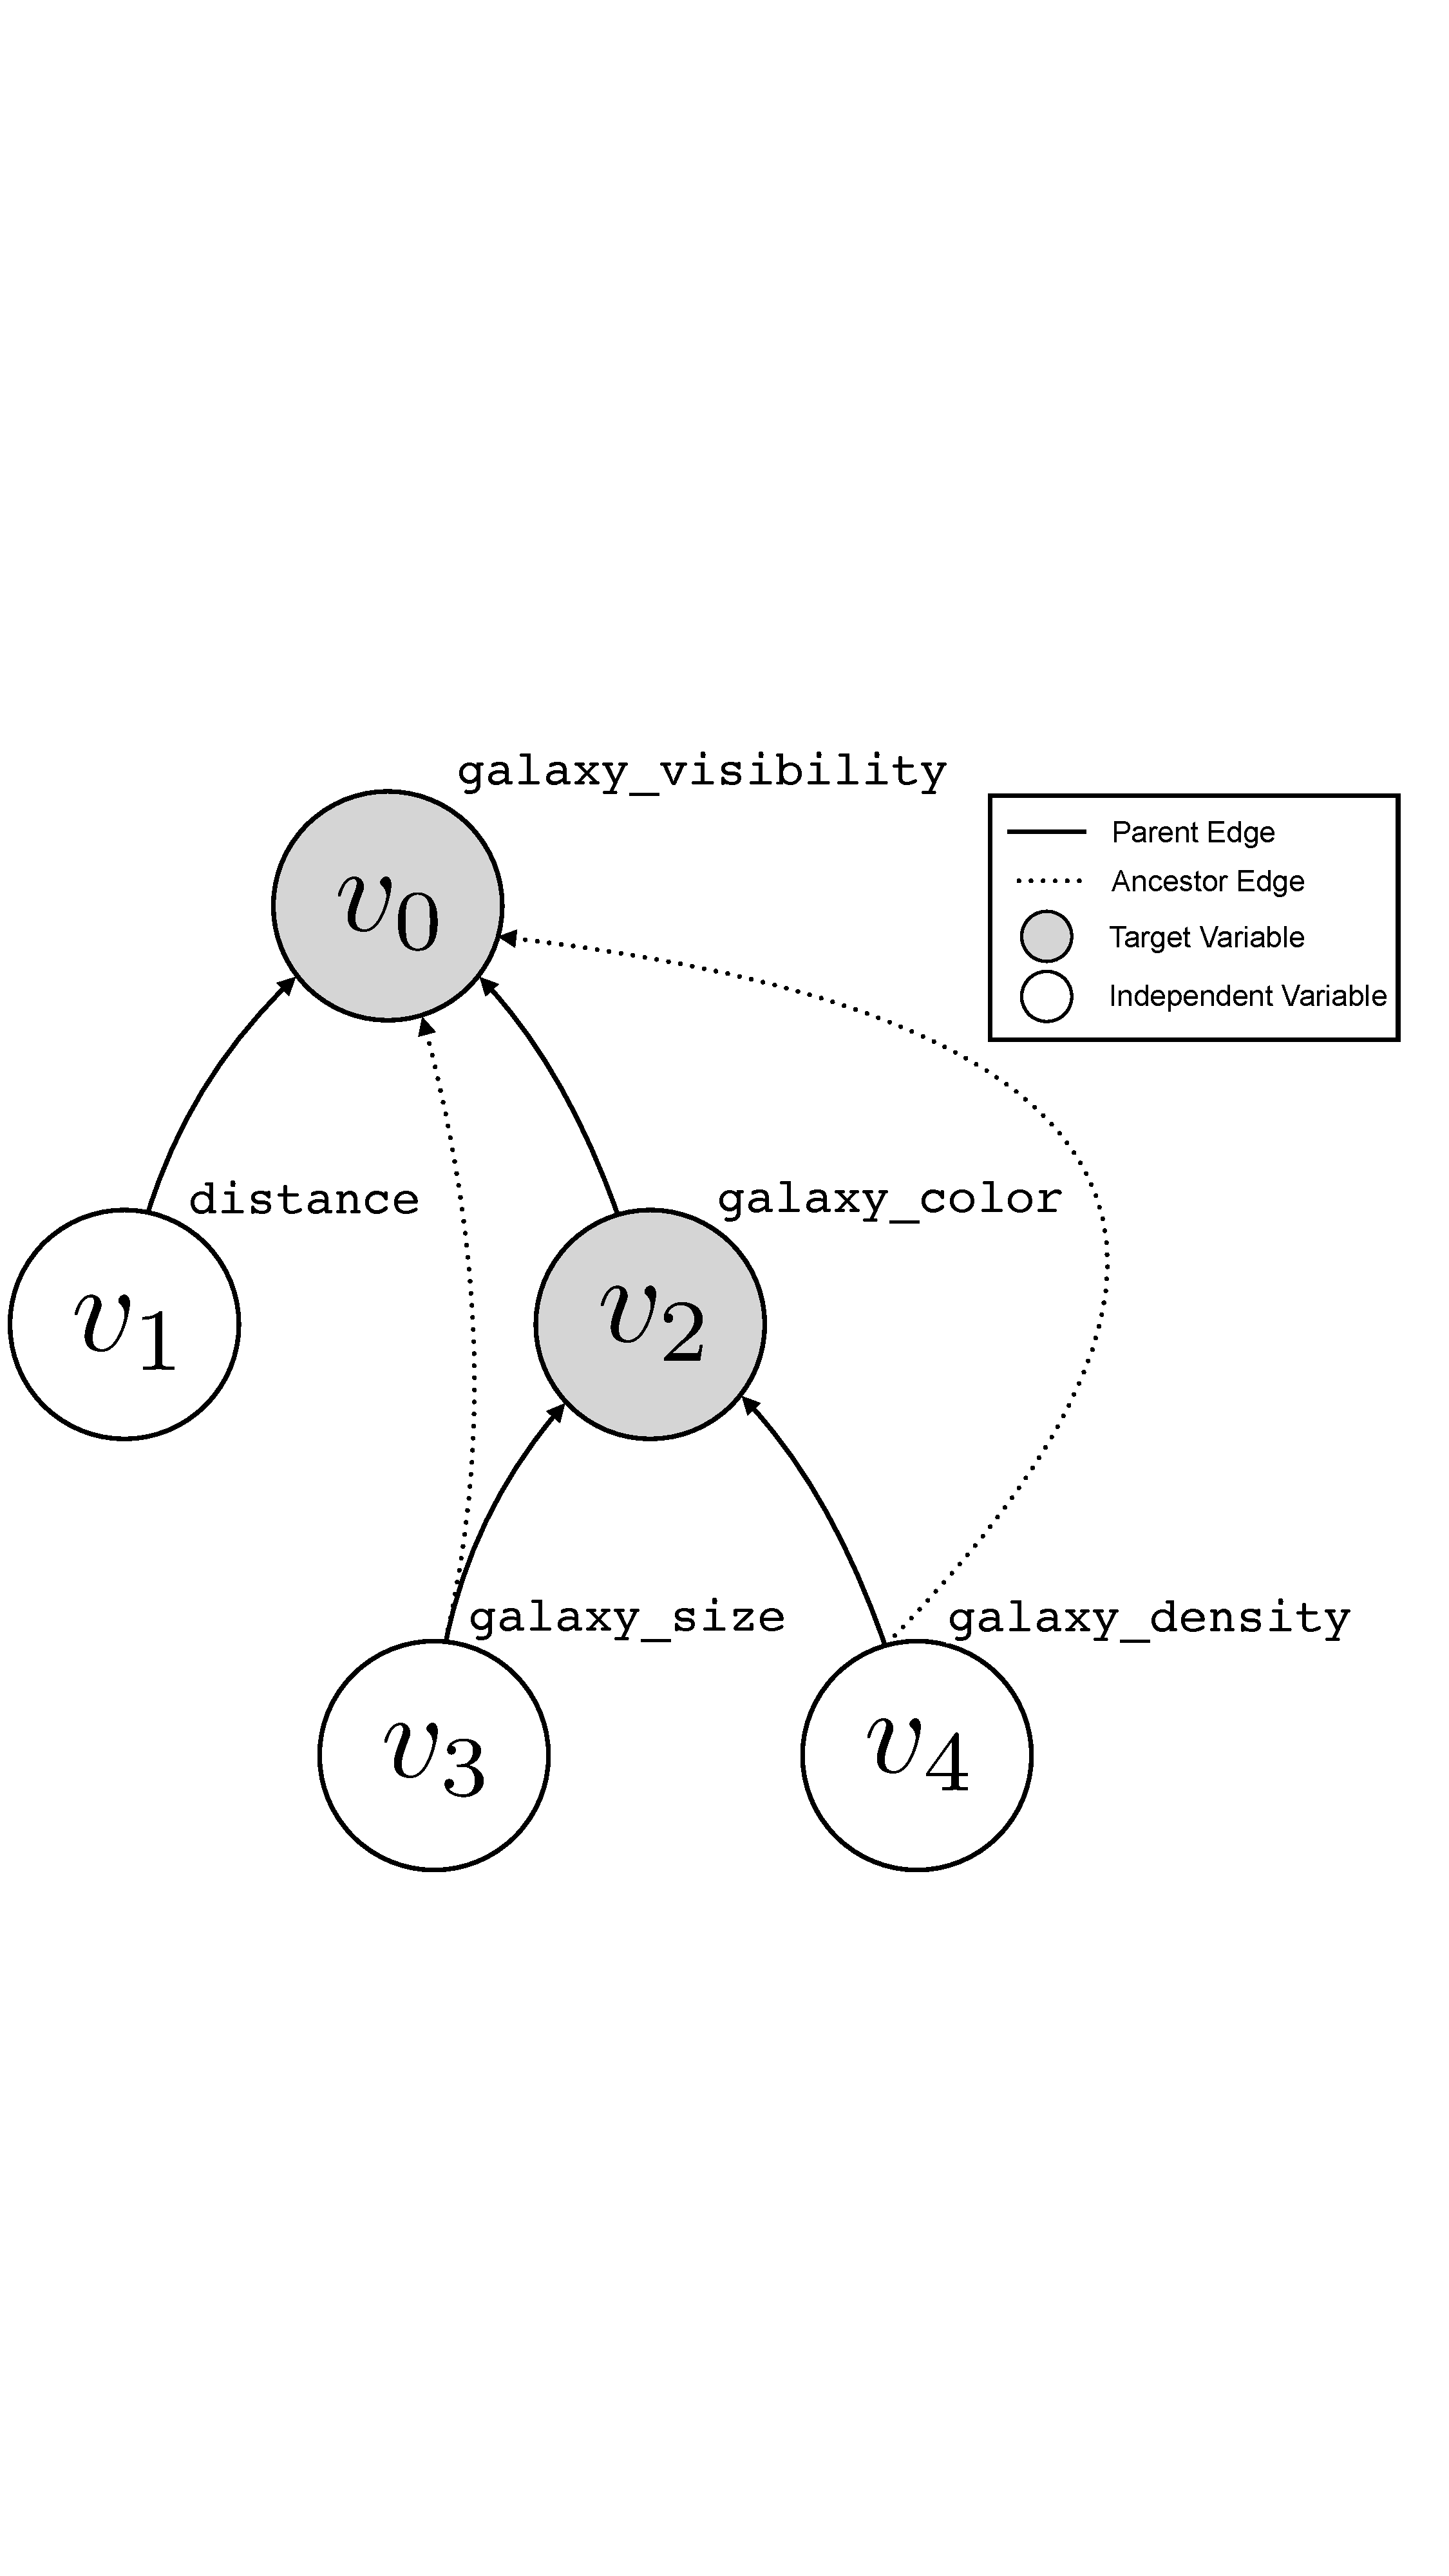
\includegraphics[trim=0 0 0 0, clip, width=0.9\linewidth]{figures/semantic_tree.pdf}
%   \caption{Hypothesis Semantic Tree}
%   \label{fig:semantic_tree}
% \end{wrapfigure}





Table~\ref{tab:real-stat} shows the diversity of tasks both in train and test split for \real{}. Most importantly, the benchmark incorporates 114 (4 + 110) tasks that require more than one related datasets
% \ashish{why `file'? it isn't quick more than one dataset?}
to be analyzed, with a maximum of 6 datasets 
% \ashish{ok, so a file is probably isn't quite a dataset. is a single dataset split into 6 files, like a relational database, for efficient storage / cleaner structure? either way, need some connection between datasets (mentioned earlier) and files (mentioned here)}
for a task. Each workflow within the dataset can be viewed as a composition of unit actions---such as code generation for statistical tests---that LLMs excel at, showing how our tasks require the chaining of such atomic actions to address complex scenarios for data-driven discovery. We measure the complexity of these workflows by quantifying the number of unit actions involved, referring to this as the \emph{workflow length}, whose distribution can be seen in Fig~\ref{fig:analysis}.



%Analysis of domains, workflows, and difficulty. Multiple datasets. How each workflow can be seen of compositions of unit actions that LLMs are known to be good at (for e.g., code generation for average calculation, etc.). This shows our tasks require chaining of such atomic actions.


%Diversity of domains - sociology, economics, ecology, biodiversity, public health, archaeology, reproducibility in science 

%Diversity of data - csv, txt, stata. Number of input files, ranging from 1 to 6 - where analysis of 6 files are needed etc. 

%Diversity of workflows - depth and complexity analysis from the execution workflow length 

%Diversity of data transformation needed - complex NLS transformation, to meta-regression joining to 6 levels of files/ joins

%Diversity of ML/ stats techniques - regression, interaction variable, PCA, quantile regression, gini coefficient, time series analysis, visual chart interpretation, meta-regression, econometric modeling, pollen modeling, ecological modeling

%Diversity of hypotheses types

% \harshit{Post masking and query formation, we also need to verify that the question does not entail any other answer, especially true for high level context and variable questions.}

\subsection{\synth: Generating data-driven hypotheses using LLMs}
% \subsection{\textsc{Synth}: Synthetics Variations in Data-driven Hypotheses}
To scale data collection, we next introduce a supplementary benchmark,
which is synthetically constructed to enable controlled model evaluations. 
% and (2) serve as training data for improving models.
Our goal is to reverse-engineer the process of hypothesis discovery to synthesize datasets and discovery tasks of varying difficulty that require analysis workflows similar to those in the real-world benchmark. 
Our approach leverages the broad pre-trained knowledge of LLMs in four stages:

% \begin{enumerate}[left=2pt, itemsep=0.1pt]
\textbf{Domain sampling:} First, we prompt the model to generate a list of diverse topics or \emph{domains} along with their natural language descriptions. E.g., 
% \ashish{general note: `e.g.' already stands for `for example'. So just say ``E.g., ...'' rather than ``For e.g., ...'' here and at various other places}
``Ancient architecture'' $\rightarrow$ ``Related to historic buildings, architectural marvels, and ancient construction techniques''.

\textbf{Semantic tree construction:} For each domain, we then build a semantic tree $\mathcal{T}_h$,
% \footnote{We drop subscript $h$ from $\mathcal{T}_h$ when it is obvious from the context.}
recursively deriving nodes starting from a primary hypothesis $h$. Specifically, we prompt the model with the domain and a sampled real-world workflow (e.g., ``within-cluster analysis'') to generate a hypothesis and its target variable.
% \footnote{Note that variables in the semantic tree and columns in a dataset have a one-to-one correspondence.}
% , e.g., (``Structures with a base width to height ratio greater than 5:1 are more likely to involve higher material usage due to construction techniques required for supporting wider bases'', $\texttt{material\_usage}$). 
Setting the target variable as root, we then derive child nodes by generating the independent variables required to verify $h$ using $\mathcal{V}(\cdot)$.
% \footnote{In practice, with probability 0.6, we choose whether a node is derived further or marked as a leaf.} using concepts from the generated hypothesis.
% constructing new child nodes to a maximum tree depth of $3$. 
We operationalize this by generating a column name and description for each child node (along with a data type and range) and a pandas expression\footnote{The pandas expression encodes the structured hypothesis $\psi(c,v,r)$.} \citep{mckinney-proc-scipy-2010} over only independent variables in $\mathcal{T}_h$ such that its execution results in the target variable. We repeat this with each leaf in $\mathcal{T}_h$ as the root of a new semantic sub-tree, generating intermediate hypotheses and a new set of variables until the desired height of $\mathcal{T}$ is reached.\footnote{In practice, with probability 0.6, we choose whether a node is derived further or marked as a leaf.}
% \footnote{This expression jointly captures the context, variable, and relationship dimensions of the hypothesis, i.e. $\psi(c,v,r)$.}. 
We also generate a set of distractor columns disjoint from nodes in $\mathcal{T}$, thus resulting in a synthetic semantic forest $\mathcal{F}$.

\textbf{Data generation:} We then construct a task dataset $D:=\{\mathbf{x}_i\}_{i=1}^m$ by generating synthetic data in a bottom-up manner (i.e., from leaves to root) for each node in $\mathcal{F}$. Starting with various sampling strategies for leaf nodes (see more in Sec~\ref{sec:synth}),
% for each nodes are explained in 
% For leaves, we use different sampling strategies based on the data type. 
% Specifically, for categorical nodes, we sample instances with replacement from the range of allowed values, whereas for numeric, we first select a distribution (e.g., normal) and its parameters based on the specified range and then perform sampling. 
for each subsequent level in $\mathcal{F}$, we create new columns for nodes by simply executing their pandas expressions.
% \footnote{The expression is guaranteed to only have variables already generated due to the bottom-up construction.}. 
% To recover from any execution errors, we additionally use a self-refine \citep{madaan2023selfrefine} approach to generate new pandas expressions guided by the execution error logs. 
Finally, to mimic real-world challenges in data collection, we probabilistically perturb each instance $x \in \mathbf{x}_i$ 
% with $0.3$ 
% \tushar{seems high. Can it be grounded with any of the real benchmarks?} \dhruv{This would be nice but we don't have support for this in the real-data since the two sets were developed in parallel.} 
% probability 
by adding noise or dropping values 
% \tushar{would you lose 15\% of the data?} \dhruv{The implementation is that every \textit{cell} in the dataset has a 30\% chance of being perturbed, so we do lose/noise 30\% of cells on average in the full dataset, but not entire rows.} 
to create missing data\footnote{Each value is noised independently; therefore, each row has sufficient true data useful for discovery.}. 
Note that at this stage, $D$ contains a column for each node in $\mathcal{F}$.

\textbf{Task generation:} For each internal node $h$ in $\mathcal{F}$, we now create multiple task datasets $D_h^{(l)}$ from $D$, varying the difficulty of the discovery task based on the path length $l$ between $h$ and the observed independent variables in $\mathcal{F}$. 
% Intuitively, as $l$ increases, an agent must infer more intermediate hypotheses to reach the target, thus making the discovery task more difficult. To create $D_h^{(l)}$, we simply mask the columns in $D$ that correspond to nodes in $\mathcal{F}$ that are within a distance of $l$ to $h$.
Finally, we follow the same strategy for goal formulation as \real{}.
% prompt the model to generate a query for each task.
We generate 903 tasks over 48 diverse domains and assign them to train, dev, and test sets using a 60/20/20 split, where each task is additionally tagged with a difficulty level from 1-4. While we evaluate our agents on the test, the training set can serve as supervised data for improving models. 


\subsection{Evaluation}
We evaluate task performance by measuring the alignment of the predicted and gold hypotheses in natural language.\footnote{We deliberately take an outcome-based approach as $> 1$ discovery path may lead to the same hypothesis.} We take inspiration from recent works in LLM benchmarking \cite{Shashidhar2023DemocratizingLA,Zeng2023EvaluatingLL,Yuan2023EvaluatingIL,Fu2023GPTScoreEA,alpaca_eval,wildbench2024} and design a model-based evaluation strategy using \texttt{gpt-4-preview-0125} as the \emph{evaluator}, conditioned on our structured formalism of data-driven hypotheses.
% \pete{Add a sentence on the i/o behavior of the evaluator, e.g., "The inputs to the evaluator are two (parts of) hypotheses to compare, and the output is a number (?) between 0 and 1 (???)"} \bodhi{it's not a one-shot prompt or one LLM-call. At the end of the process, we get a score HMS, as we describe below.}

% and construct
% Model-based evaluation has become an integral part of LLM benchmarking and reward modeling. \bodhi{cite}
% % refer: https://arxiv.org/pdf/2404.13076v1
% To accommodate the free-form nature of our target hypotheses and still evaluate generated ones robustly, we use the structured formalism of data-driven hypotheses combined with model-based evaluation. Our evaluation is outcome-based, i.e., we do not differentiate hypotheses derived using different workflows. We use \texttt{gpt-4-preview-0125} as our \emph{evaluator}.

Recall the propositional form $h := \phi(h_1,\ldots,h_n)$ of a hypothesis $h$ that decomposes it into sub-hypotheses. We first use our GPT-4 based evaluator to independently decompose the gold ($h^g$) and predicted ($h^p$) hypotheses into their respective sub-hypotheses $\{h^g_i\}_{i=1}^n$ and $\{h^p_j\}_{j=1}^m$,
% where each sub-hypothesis $h_k$ itself is, in turn, expressed as a declarative sentence $\psi(c_k, v_k, r_k)$ encoding the
asking it to also identify, for each sub-hypothesis $h_k$,
its context, variables, and relationship dimensions (prompt in \Cref{list:decompose}). Given this structured representation of the gold and predicted hypotheses, we then compute a \textbf{hypothesis match score (HMS)}, which measures the degree to which two hypotheses align on each dimension, as follows.


% We then use a facet-based evaluation over $c_i, v_i, r_i$, which measures task performance using the prediction accuracy of each dimension. 
% \ashish{Updated this paragraph + the notation:}
To compute HMS, we match each predicted sub-hypothesis $h^p_j$ with a gold sub-hypothesis $h^g_i$ when their contexts are judged as equivalent by our GPT-4 based evaluator (prompt in \Cref{list:match}).\footnote{Note that at most one gold sub-hypothesis is matched with a predicted sub-hypothesis.} Let $M$ denote this set of context-matched pairs of predicted and gold sub-hypotheses. At this point, treating each sub-hypothesis context as a single unit, we can compute an F1 score, $\contextscore$, capturing how aligned the $n$ contexts of sub-hypothesis of $h^g$ with the $m$ contexts of sub-hypotheses of $h^p$. Then, for each matched pair of sub-hypotheses, we measure how well the variables and relations align, using an F1 score for the variables ($\variablescore$) and an accuracy score for the relation ($\relationscore$).
% to measure alignment along the context dimension and alignment scores for the variable and relationship dimensions over only the sub-hypothesis pairs in $M$.
Specifically, for each sub-hypothesis pair in $M$, we extract the set of interacting variables
% \ashish{it's not totally clear what this means; can we point to the exact prompt for this too?}
in the gold and predicted sub-hypotheses using the GPT-4 based evaluator (prompt in \Cref{list:variable}). We compute the alignment between these two sets of variables as an F1 score, $\variablescore$, similar to how $\contextscore$ was computed. For relationships, we compute relationship accuracy with reference to the relationship between the gold variables
% \ashish{currently it's unclear what relation you look for and evaluate --- is it between gold variables? or variable-agnostic? probably the former (depends on the exact prompt used). needs clarity. a pointer to the prompt would help, again.}
($\relationscore$) based on evaluator judgments using the following scoring heuristic: $100$ if there is an exact match of the relation, $50$ when the predicted relationship is broader than the gold relationship but encompasses it, and $0$ otherwise (prompt in \Cref{list:rel}).
% \ashish{this leaves open the case of the predicted relation being more specific than gold. Should we change to `$0$ otherwise', if that's what you do?}.
Finally, we compute HMS $\in [0, 100]$ as the average alignment of the variable and relationship dimensions over context-matched sub-hypotheses, weighted by the overall context alignment:
\[
    \hmsscore(h^p, h^g) = \contextscore(h^p, h^g) \times \frac{1}{|M|} \sum_{i=1}^{|M|} \Big( \variablescore(h^p_i, h^g_i) \times \relationscore(h^p_i, h^g_i) \Big)
\]

% At this point, we derive a composite accuracy score for each matched pair as $v_{\text{F1}} \times r_{\text{acc}}$ multiplied by the context matching score for the matched pairs, which is always $1$. \bodhi{why product}
% We compute a recall score for context ($c_{\text{recall}}$) using the number of predicted (sub)hypotheses of relevant context, penalizing the overgeneration of hypotheses not relevant to the discovery goal.

% We then use a facet-based evaluation over $c_i, v_i, r_i$, which measures task performance using the prediction accuracy of each dimension. First, for every predicted sub-hypothesis $h_{\text{p}, i}$, we match it with only one subsequent gold sub-hypothesis $h_{\text{g}, j}$ when their contexts exactly match according to the evaluator. Let us denote the set of matched context pairs as 
% % $C_{\mathrm{matched}}$.
% $H_{c\text{-matched}}$. 
% We compute a recall score for context ($c_{\text{recall}}$) using the number of predicted (sub)hypotheses of relevant context, penalizing the overgeneration of hypotheses not relevant to the discovery goal.   

% Now, for each matched pair of generated and gold sub-hypothesis, we evaluate the two remaining dimensions. For variables, the evaluator systematically returns the number of variables used and mentioned in both the gold and generated hypothesis, from which an F1 score is computed ($v_{\text{F1}}$). For comparing relationships in the gold and generated sub-hypothesis, the evaluator scores 1 when the relationships are exactly similar, scores 0.5 when the generated relationship is more general than the gold relationship, and 0 when they are different, resulting in an accuracy score $r_{\text{acc}}$. At this point, we derive a composite accuracy score for each matched pair as $v_{\text{F1}} \times r_{\text{acc}}$ multiplied by the context matching score for the matched pairs, which is always $1$. \bodhi{why product}

% From this, we derive our final score as:
% \[
% \text{final score} = c_{\text{recall}} \times \frac{1}{|H_{c\text{-matched}}|} \sum v_{\text{F1}} \times r_{\text{accuracy}} \quad \forall (h_{\text{p}, i}, h_{\text{p}, j}) \in H_{c\text{-matched}}
% \]
% \bodhi{does the avg capture context precision?}

% In addition to the hypotheses, we also provided the gold and predicted workflow (where available) to disambiguate the information present in the hypothesis, such as context may not be clearly expressed in the hypothesis but can be clearly gleaned from the workflow.\dhruv{Should we move this last paragraph to appendix?}
% \bodhi{TBD correlation with human eval vs model-based eval} 
 



% GPT-4 based eval.

% Entailment-based evaluation along different dimensions

% We perform GPT-4 based evaluation comparing the model-generated hypothesis (HypoGen) with the gold hypothesis in our dataset (HypoGold) in terms of 3 dimensions: Context, Variables, and Relation. We compute a score between 0-1 for each dimension based on the GPT-4’s answer to a multiple-choice question listed below. The final eval report would consist of scores as well as NL explanations generated by GPT-4 for each of the dimensions. 

% E.g. for a hypothesis: From 1995 to 2009, the number of sandhill cranes around the tundra (Indigilka River) surged by an astounding ~10X
% Context refers to the stratification of the data under which the given hypothesis is True. e.g. "From 1995 to 2009"
% \\
% Q: Is HypoGen defined in the same context as HypoGold?
% A) very different   B) overlapping with HypoGold   C) HypoGen subset of HypoGold  D) same 
% Variables refer to the set of variables (either dependent or independent) that are mentioned in the  hypothesis e.g. number of sandhill cranes, location
% \\
% Q: Does HypoGen use the same variables as the one used in HypoGold?
% A) different    B) HypoGen has variables not in HypoGold C) HypoGold has variables not in HypoGen  D) same
% Relation refers to the form of the relation between the variables e.g. surged by ~10x.
% \\
% Q: Does HypoGen exhibit the same relation between variables as HypoGold?
% A) very different    B) HypoGen is more general than HypoGold   C) HypoGen is more specific than HypoGold  D) same
